\chapter{Estado del Arte}

\section{Estimación de la edad}
\label{traditional_labeling_methods}
La estimación de la edad, al ser un componente clave en la determinación del PB, ha captado un creciente interés por parte de la comunidad científica desde el siglo pasado, evidenciando una tendencia al alza en el número de publicaciones. En la Figura \ref{fig:scopusData} se muestra la evolución del volumen de publicaciones indexadas en la base de datos \textit{Scopus} que hacen referencia tanto a la AF como a la estimación de edad por medio de la cadena de búsqueda \ref{code__scopus_af}, registrándose un total de 1,451 trabajos desde el siglo XX.

Sin embargo, y en línea con lo ya mencionado respecto a la limitada sofisticación tecnológica de esta disciplina, el número de publicaciones que integran técnicas de IA es considerablemente más reducido, al realizarse la consulta con la cadena \ref{code__scopus_af_ai} se identifican 76 artículos.

Finalmente, al acotar aún más la búsqueda a estudios que combinen IA con modelos tridimensionales para la estimación de edad mediante AF con la cadena \ref{code__scopus_af_ai_3d}, se obtienen únicamente ocho artículos. Esta escasa representación refuerza el carácter novedoso y pionero del presente trabajo.

\begin{lstlisting}[caption={Cadena de búsqueda de \textit{Scopus} para obtener publicaciones de AF que referencian la estimación de la edad.}, captionpos=b, label=code__scopus_af, style=Consola]
(TITLE-ABS-KEY (forensic AND anthropology AND age AND estimation))
\end{lstlisting}
            
\begin{lstlisting}[caption={Cadena de búsqueda de \textit{Scopus} para obtener publicaciones de AF que referencian la estimación de la edad y hacen uso de alguna técnica de IA}, captionpos=b, label=code__scopus_af_ai, style=Consola]
(TITLE-ABS-KEY (((deep AND learning) OR (machine AND learning) OR (soft AND computing) OR (artificial AND intelligence) OR (data AND mining)) AND forensic AND anthropology AND age AND estimation))
\end{lstlisting}
            
\begin{lstlisting}[caption={Cadena de búsqueda de \textit{Scopus} para obtener publicaciones de AF que referencian la estimación de la edad, hacen uso de alguna técnica de IA y utilizan datos 3D.}, captionpos=b, label=code__scopus_af_ai_3d, style=Consola]
(TITLE-ABS-KEY ( ((deep AND learning) OR (machine AND learning) OR (soft AND computing) OR (artificial AND intelligence) OR (data AND mining) ) AND forensic AND anthropology AND age AND estimation AND 3d))
\end{lstlisting}

\begin{figure}[h]
    \centering
    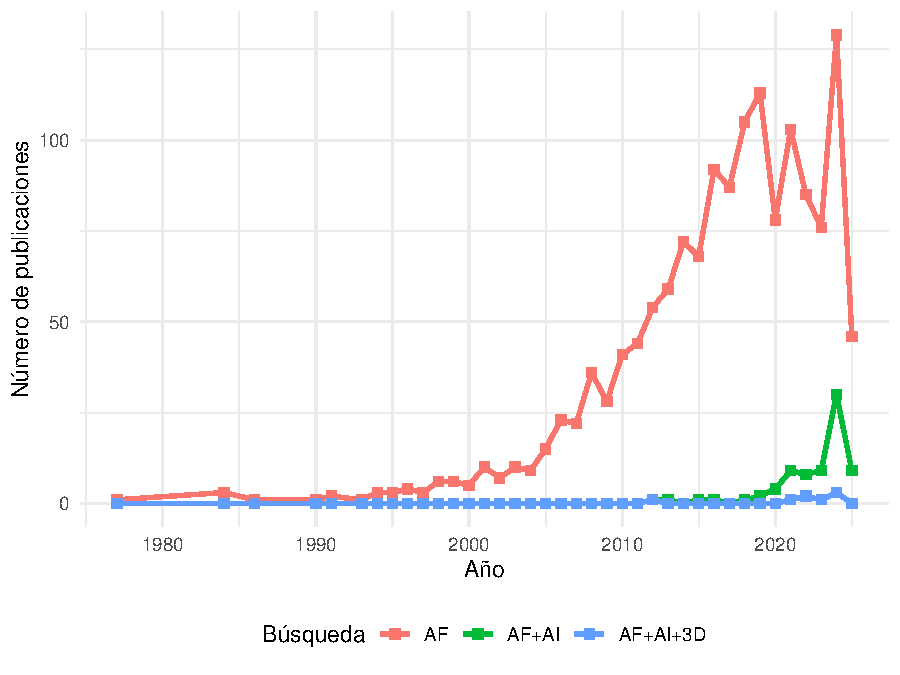
\includegraphics[width=\linewidth]{figures/3_sota/scopus_pubs.pdf}
    \caption[Publicaciones por año de AF, AF+IA y AF+IA+3D en Scopus]{Número de publicaciones en \textit{Scopus} en función del año a fecha de 13/07/2025. En {\color{Red} \textbf{rojo}} se muestran las publicaciones que mencionan AF y la estimación de la edad (1,451 publicaciones), en {\color{LimeGreen} \textbf{verde}} aquellas que adicionalmente mencionan alguna técnica de IA (76 publicaciones) y en {\color{Blue} \textbf{azul}} aquellas que también mencionan el uso de 3D (8 publicaciones).}
    \label{fig:scopusData}
\end{figure}

En las siguientes subsecciones primero se presenta brevemente el estado del arte de los métodos estimación de edad tradicionales. Posteriormente se presentan los métodos de estimación automáticos haciendo uso de la sínfisis del pubis y finalmente, el estado del arte del procesamiento de datos 3D por DL.

\subsection{Métodos tradicionales para restos óseos}
\subsubsection{Suturas craneales}
A lo largo del tiempo se han propuesto distintos métodos para evaluar el grado de osificación de las articulaciones fibrosas del cráneo, conocidas como suturas craneales. Entre los más relevantes se encuentran los de Acsádi y Nemeskéri \cite{acsadi1970history}, Meindl y Lovejoy \cite{meindl1985ectocranial}, Mann \cite{mann1991maxillary} y Perizonius \cite{perizonius_closing_1984}. En general, estos métodos se basan en la observación macroscópica del cierre de las suturas, clasificando su estado en diferentes categorías que luego se traducen en una estimación de edad. No obstante, la precisión de esta técnica ha sido ampliamente cuestionada, considerándose insuficiente para un uso práctico en AF \cite{franklin_forensic_2010}, salvo cuando se emplea de manera complementaria junto con otros métodos basados en estructuras óseas distintas o con el uso de tomografías axiales computarizadas para aumentar su precisión \cite{ruengdit2020cranial}.

\subsubsection{Costillas}
El método más ampliamente utilizado es el desarrollado por İșcan y Loth \cite{icscan1984age, icscan1985age}, que se centra en el análisis del extremo ventral de la cuarta costilla mediante un sistema de nueve fases que describen el proceso de envejecimiento de esta estructura. La evaluación considera aspectos como la forma, la textura y la calidad del hueso, que permiten asignar la muestra a una fase determinada, la cual está vinculada a un rango específico de edad. Sin embargo, esta técnica presenta limitaciones derivadas de sesgos poblacionales, variabilidad intra- e interobservador y una reducida reproducibilidad \cite{fanton2010critical, hartnett2010analysis}. Con el fin de solventar estas limitaciones, se han propuesto mejoras basadas en enfoques de estadística bayesiana \cite{munoz_sex_2018} y en la aplicación de tomografía axial computarizada \cite{blaszkowska2019validation}.

\subsubsection{Cara auricular del ilion}
Existen diversos métodos que emplean el desgaste de la cara auricular del ilion, situada en la pelvis, como indicador de edad. El primero fue propuesto por Lovejoy \cite{lovejoy1985chronological}, y posteriormente ampliado en los métodos de Buckberry y Chamberlain \cite{buckberry_age_2002} y de Osborne \cite{osborne_reconsidering_2004}. La elección de esta zona se debe a su resistencia al daño post-mortem y a la estabilidad de la articulación, lo que provoca que el patrón de desgaste se desarrolle de forma relativamente constante a lo largo de la vida. Sin embargo, la precisión de las estimaciones es limitada, ya que las categorías establecidas son demasiado amplias y se solapan, además de estar afectadas por sesgos poblacionales \cite{falys2006auricular, michopoulou2017auricular}. Con el objetivo de mejorar la fiabilidad de este enfoque, se han incorporado técnicas de imagen avanzadas, como la tomografía axial computarizada \cite{warrier_applicability_2024, villa2013reliability}.

\subsection{Métodos tradicionales utilizando la sínfisis del pubis}
Los métodos de Todd y de Suchey-Brooks son los más empleados en AF para la estimación de la edad. Ambos procedimientos consisten en examinar detalladamente la superficie de la sínfisis del pubis, evaluando el desgaste que ocurre a medida que el individuo envejece (véase Tabla \ref{table:themBones} y \ref{themBomes:visualExample}), y clasificando dicho desgaste en distintas fases según los rangos establecidos por cada método, los cuales se presentan en las Tablas \ref{table:age_todd_} y \ref{table:age_suchey_brooks}.

\begin{table}[h]
\centering
\resizebox{\textwidth}{!}{%
\begin{tabular}{|
>{\columncolor[HTML]{D33333}}c |c|c|c|c|c|c|c|c|c|c|}
\hline
{\color[HTML]{FFFFFF} \textbf{Rango de Edad}} & I & II & III & IV & V & VI & VII & VIII & IX & X \\ \hline
{\color[HTML]{FFFFFF} \textbf{Etapa}} & 18-19 & 20-21 & 22-24 & 25-26 & 27-30 & 30-35 & 35-39 & 39-44 & 45-50 & 50+ \\ \hline
\end{tabular}%
}
\caption{Rangos de edad del Método de Todd.}
\label{table:age_todd_}
\end{table}

\begin{table}[h]
\centering
\begin{tabular}{|
>{\columncolor[HTML]{D33333}}c |c|c|c|c|c|c|}
\hline
{\color[HTML]{FFFFFF} \textbf{Etapa}} & I & II & III & IV & V & VI \\ \hline
\cellcolor[HTML]{D33333}{\color[HTML]{FFFFFF} \textbf{Rango de Edad}} & 15-23 & 19-34 & 21-46 & 23-57 & 27-66 & 34-86 \\ \hline
\end{tabular}
\caption{Rangos de edad del Método de Suchey-Brooks.}
\label{table:age_suchey_brooks}
\end{table}

Estos métodos se consideran generalmente los más precisos dentro del contexto forense. No obstante, diversos autores advierten sobre la necesidad de aplicarlos con cautela debido a sus limitaciones intrínsecas \cite{priya2017methods}. Actualmente, la disponibilidad de imágenes provenientes de tomografías computarizadas ha permitido aplicar los métodos sobre modelos volumétricos, replicando de forma virtual el análisis que tradicionalmente se realiza sobre el hueso físico. Estudios recientes \cite{wade2011preliminary,villa2013forensic,lottering2014morphometric,lopez2015image} han aprovechado esta tecnología para examinar cambios en la densidad ósea interna asociados al envejecimiento, contribuyendo así a refinar las estimaciones. A pesar de estas mejoras, la práctica sigue dependiendo de la evaluación de características morfológicas subjetivas, lo que provoca que las estimaciones finales estén fuertemente condicionadas por la experiencia del perito, más que por un análisis objetivo y sistemático, comprometiendo tanto la precisión como la confiabilidad del proceso \cite{garvin_current_2012}.

\subsection{Métodos automáticos utilizando la sínfisis del pubis}

Los primeros intentos por reemplazar los métodos subjetivos en la estimación de edad a partir de la sínfisis del pubis surgen a inicios de la década de 2010 con el estudio realizado por Biwasaka et al. \cite{biwasaka2013three}. En dicho trabajo se calcula analíticamente la curvatura media de la superficie de la sínfisis del pubis, obtenida mediante escaneo 3D, para evaluar el grado de concavidad o convexidad del hueso en relación con los intervalos de edad definidos por el método de Suchey-Brooks. Aunque se utilizó una muestra de 145 huesos y se concluye que existe una relación entre las fases del método y la curvatura, el estudio no reporta métricas estadísticas cuantitativas que respalden los hallazgos.

Villa et al. \cite{villa2015quantitative} amplían el enfoque anterior al definir cinco variables derivadas del análisis de curvatura: la media del valor absoluto de la curvatura, el 10\% de curvaturas más altas, el 10\% más bajas, el porcentaje de superficie con curvaturas mayores que cero (regiones convexas) y el porcentaje con curvaturas entre $-0.01$ y $0.01$ (regiones planas). Se emplearon dos conjuntos de datos: uno con 24 huesos, que arrojó una correlación de Spearman moderada a fuerte ($\rho=0.60-0.93$), y otro con 98 huesos, con correlaciones más débiles ($\rho=0.29-0.51$), comparables a los valores alcanzados por métodos manuales, lo cual demuestra el potencial de este enfoque.

En Slice y Algee-Hewitt \cite{slice2015modeling} se introdujo una métrica denominada \textit{Slice Algee-Hewitt Score} (SAH-Score), basada en un análisis de componentes principales aplicado a los vértices de mallas 3D de la sínfisis del pubis. Esta métrica cuantifica la complejidad superficial del hueso y se utiliza como predictor en un modelo de regresión lineal para estimar la edad. Con una muestra de 41 huesos, se obtuvo un error cuadrático medio (RMSE) de 17.15 años, con predicciones que coinciden razonablemente con los intervalos del método de Suchey-Brooks.

Stoyanova et al. \cite{stoyanova2015enhanced} emplean el algoritmo \textit{Thin Plate Splines} para estimar la energía de flexión (\textit{bending energy}, BE) requerida para transformar una superficie plana en la forma tridimensional del hueso. Esta métrica se usa en un modelo de regresión lineal entrenado con 44 mallas, obteniendo un RMSE de 19 años. En un trabajo posterior \cite{stoyanova2017computational}, los autores combinan múltiples características (SAH-Score, BE y curvatura del borde ventral) para entrenar un modelo de regresión multivariable con 93 muestras, logrando un RMSE entre 13.7 y 16.5 años.

Villar et al. \cite{villar2017first} utilizan Árboles de Decisión Difusos (\textit{Fuzzy Decision Trees}) para generar reglas que permitan clasificar los huesos en los intervalos de edad del método de Todd, usando 74 muestras etiquetadas por dos expertos. El modelo alcanza un error absoluto medio (MAE) de 1.68 años respecto al intervalo correspondiente, aunque el número reducido de muestras impidió cubrir todos los rangos de edad.

En Gámez-Granados et al. \cite{granados} se propone un sistema explicable basado en reglas utilizando el clasificador ordinal NSLVOrd \cite{gamez2016ordinal}, el cual clasifica 892 muestras de sínfisis del pubis dentro de los 10 intervalos definidos por Todd, utilizando las nueve características tradicionales etiquetadas por expertos. Aunque el enfoque es de clasificación, puede adaptarse para predecir directamente la edad. El modelo reporta un RMSE de 12.34 años y un MAE de 10.38 años.

Kotěrová et al. \cite{kotverova2018age} exploran nueve métodos de regresión aplicados a características extraídas manualmente por expertos. Con una muestra de 941 huesos, la regresión lineal múltiple ofrece el mejor desempeño, con un RMSE de 12.1 años y un MAE de 9.7 años. En una extensión del estudio \cite{koterova_computational_2022}, se incorporan mallas 3D y se introducen dos nuevos enfoques: uno que caracteriza la superficie del hueso mediante la energía de Dirichlet, y otro basado en una CNN entrenada con múltiples proyecciones 2D del modelo 3D. Los mejores resultados obtenidos son un MAE de 11.7 y 10.6 años, respectivamente.

Bermejo et al. \cite{bermejo_interpretable_2025} proponen un método semi-automático e interpretable, basado en regresión simbólica obtenida mediante Programación Genética, utilizando como entrada las nueve características del método de Todd. El mejor modelo generado reporta un MSE de 10.81 años y un MAE de 8.55 años. Aunque estos resultados representan una mejora frente al método propuesto por Kotěrová, los autores consideran ambos enfoques como equivalentes y complementarios, dado que el modelo de Bermejo requiere el etiquetado experto de las características, mientras que el de Kotěrová es completamente automático.

Finalmente, en Irurita et al. \cite{irurita2025pubic} se evaluó la viabilidad del modelo de XAI propuesto en \cite{granados} desde la perspectiva de la AF. Para ello, se elaboró un nuevo atlas textual y visual con el objetivo de facilitar la anotación precisa de las características morfológicas de la sínfisis del pubis. Este recurso fue empleado por dos expertos y dos novatos en un ejercicio de identificación de dichas características, permitiendo analizar tanto el error intra- como interobservador. Además, se evaluó el impacto de estas anotaciones en la estimación de edad mediante el modelo XAI, comparando los rangos de edad de Todd obtenidos por el sistema con los generados a partir de las observaciones humanas usando el atlas. Los resultados mostraron que tanto el modelo como los participantes alcanzaron un \textit{accuracy} del 70\% en la predicción del rango de edad, lo cual sugiere que el uso de métodos automáticos representa una alternativa prometedora para mejorar este proceso. No obstante, el estudio también subraya la necesidad de que estos modelos aprendan a partir de datos provenientes de múltiples observadores, a fin de evitar la replicación de sesgos individuales en la interpretación de las características.

Los cuatro últimos estudios mencionados son los más cercanos al enfoque de este TFM. En \cite{koterova_computational_2022} se emplea una CNN para extraer automáticamente características de la sínfisis del pubis a partir de un modelo 3D, aunque con el objetivo de estimar directamente la edad, a diferencia del presente proyecto, cuyo objetivo es clasificar el hueso según las características del método de Todd. En esta línea, los trabajos de \cite{granados}, \cite{bermejo_interpretable_2025} y \cite{irurita2025pubic} sí hacen uso explícito de dichas características partiendo de información etiquetada por expertos. Estos enfoques permiten obtener reglas explicables para clasificar un hueso dentro de los intervalos de edad, o bien estimar un valor numérico de edad, pero no permiten identificar directamente las características morfológicas en la sínfisis del pubis. En este sentido, el presente trabajo se plantea como pionero, ya que, según la literatura consultada, no existe otro estudio que utilice técnicas de DL para extraer automáticamente las características de Todd a partir de modelos 3D.

\section{Representaciones 3D en \textit{Deep Learning}}
\label{3d_reprs_DL}
Como se discutió en la Sección \ref{section2:3dreps}, existen diversas formas de representar datos tridimensionales para su uso en técnicas de DL. En esta sección se evalúa cuál de estas representaciones resulta más adecuada para el presente proyecto, así como los avances recientes asociados a la misma.

En primer lugar, se descartan las representaciones que convierten los datos a formatos 2D, como proyecciones o vistas múltiples, ya que se desea aprovechar al máximo la riqueza de detalle que ofrecen los datos 3D sobre las superficies de los objetos. Este tipo de representación provoca la pérdida de información, especialmente en zonas complejas de la malla donde pueden producirse oclusiones. De manera similar, se descarta la representación RGB-D, que tampoco captura la complejidad completa del modelo tridimensional.

Las nubes de puntos, aunque tridimensionales, resultan insuficientes para este proyecto, pues generan ambigüedades a la hora de reconstruir la superficie de la malla, particularmente en escenarios que requieren un alto nivel de detalle. Los descriptores 3D, que generan \say{firmas} o representaciones compactas de la malla, también se consideran inadecuados, ya que pierden información topológica crítica. Por la misma razón, se descartan las representaciones basadas en grafos, que requieren transformaciones intermedias de la malla 3D.

Las representaciones volumétricas, como los vóxeles o los árboles octales, presentan limitaciones importantes debido a su ineficiencia computacional y alto consumo de recursos. Resulta impracticable utilizarlas al nivel de detalle requerido para los escaneos 3D de huesos de este proyecto.

Por estas razones, se seleccionan las mallas poligonales como la representación óptima para este trabajo. Esta representación combina eficiencia y precisión: en áreas planas se emplean pocos polígonos, mientras que en zonas complejas la densidad aumenta, permitiendo capturar detalles intrincados. Además, las mallas poligonales son ampliamente utilizadas en informática gráfica, lo que ha generado un ecosistema de herramientas y algoritmos para su análisis. La mayoría de los escáneres 3D utilizados en AF generan directamente este tipo de mallas, facilitando el flujo de trabajo. Desde la perspectiva de las CNNs, las mallas ofrecen la ventaja de proporcionar información explícita sobre la conectividad de los vértices, lo que permite definir vecindarios locales de manera natural y estructurada.

\subsection{Mallas poligonales}
\label{section3:meshes}

En el trabajo pionero de Feng et al. \cite{feng2019meshnet} se propone MeshNet, el primer \textit{framework} basado en CNNs diseñado para procesar directamente mallas 3D. En este enfoque, la unidad básica de procesamiento no son los vértices ni los vóxeles, sino las caras triangulares de la malla, las cuales permiten mantener la conectividad topológica y facilitan la definición de operaciones análogas a las convoluciones en imágenes, donde los píxeles tienen vecindarios bien definidos.

Cada cara triangular es descrita por dos tipos de características, que funcionan como el análogo del valor RGB en imágenes: características espaciales y características estructurales.
\begin{itemize}
    \item Las características espaciales se calculan a partir de la posición del centroide de cada triángulo, representando su ubicación en el espacio.
    \item Las características estructurales se dividen en dos componentes: una que captura la estructura interna de la cara (por ejemplo, ángulos internos o proporciones entre lados), y otra que captura la estructura externa, que examina el vecindario local de cada cara, permitiendo aprender sobre la disposición relativa entre caras adyacentes.
\end{itemize}
Además, se redefine la operación de convolución para que trabaje de forma coherente con estas representaciones. El bloque convolucional propuesto consta de dos partes:

\begin{itemize}
    \item Una combinación de características espaciales y estructurales, que permite mezclar la posición con la forma local del triángulo.
    \item Una agregación estructural, que aprende a fusionar la información del vecindario de caras.
\end{itemize}
Ambas operaciones generan nuevas representaciones que se pasan al siguiente bloque de la red, permitiendo una jerarquía de aprendizaje similar a las CNNs tradicionales. Para la validación del modelo, se utilizó el conjunto de datos ModelNet40 \cite{wu20153d}, una base de datos ampliamente utilizada en tareas de clasificación de objetos 3D. MeshNet alcanzó un 91.9\% de precisión en la tarea de clasificación, superando a modelos basados en nubes de puntos, representaciones volumétricas y métodos basados en múltiples vistas.

En Hanocka et al. \cite{hanocka2019meshcnn} se propone otro \textit{framework} denominado MeshCNN, publicado casi en paralelo con MeshNet, con solo unos meses de diferencia. A diferencia de MeshNet, que toma como unidad básica de procesamiento las caras triangulares, MeshCNN utiliza las aristas que conectan los vértices de la malla como unidad convolucional, lo que constituye el análogo al píxel en una imagen. Cada arista es caracterizada mediante un vector de cinco componentes, compuesto por atributos geométricos que son invariantes a traslación y rotación. Esto permite realizar operaciones de convolución de manera más directa y robusta frente a transformaciones espaciales. Una de las contribuciones más importantes de MeshCNN es la implementación de una operación de \textit{pooling} adaptativo, donde la red aprende automáticamente qué regiones de la malla puede simplificar y cuáles debe preservar, optimizando así la tarea de aprendizaje. Los experimentos se realizaron en distintos conjuntos de datos, obteniendo un 98.6\% de \textit{accuracy} en SHREC30 \cite{lian2011shape} y un 92.16\% en un conjunto de cubos esculpidos con diferentes formas \cite{latecki2000shape}.

Por último, Kim y Chae \cite{kim_exmeshcnn_2022} introducen ExMeshCNN. Este \textit{framework} amplía las ideas propuestas por métodos anteriores, ya que combina la información extraída tanto de caras triangulares como de aristas. Para ello, la capa inicial de cualquier modelo basado en esta técnica incorpora dos capas que caracterizan cada cara triangular con diferentes propiedades y relaciones tanto geométricas como geodésicas. Estas capas se denominan en el artículo como \say{descriptores} y también actúan en cierto modo como filtros de convolución porque poseen parámetros entrenables, lo que le permite a los modelos amplificar o reducir la influencia de cada una de las propiedades de la cara dependiendo de la tarea que debe realizar. ExMeshCNN representa la información extraída de las caras triangulares y sus vecindarios locales como una lista unidimensional, por lo que las capas convolucionales en la red aplican directamente convoluciones 1D sobre los datos. A diferencia de MeshCNN\footnote{A pesar de la similitud en nombres pueda implicar que ExMeshCNN sea una extensión de MeshCNN, estos dos \textit{frameworks} poseen gran diferencia entre sí. Para una comparativa más detallada, ver Subsección \ref{exmeshcnn_vs_meshcnn}.}, que emplea operaciones de \textit{pooling} para aportar explicabilidad al modelo, ExMeshCNN permite aplicar técnicas como Grad-CAM gracias al uso de convoluciones 1D, lo que posibilita identificar directamente qué caras tienen mayor relevancia en la generación de una salida específica.

En los experimentos realizados con los conjuntos de datos ModelNet40 y Manifold40, ExMeshCNN alcanzó los mejores resultados reportados hasta la fecha, con 93\% y 93.4\% de \textit{accuracy} respectivamente, superando a modelos como MeshCNN y MeshNet++. De igual forma, en los conjuntos SHREC11 y el de cubos esculpidos, alcanzó un \textit{accuracy} del 100\%, posicionándose así como el \textit{framework} actual de referencia en el uso de \textit{Deep Learning} sobre mallas 3D.